\section{Défaillances de marché}

This chapter is about the \textbf{défaillances de marché} (\textit{market
failures}), in the four cases the course takes in turn: the monopole, the
externalités, the biens publics and biens communs, and the asymétries
d'information. Each case shows the market, left to itself, going wrong in a way a
diagram or an example can point to: the monopole sells less than the quantité
efficace, an externalité pulls the market's quantity away from the optimum, the
biens publics suffer from sous-investissement, and an asymétrie d'information can
make a market collapse.\\

The tools are those of the earlier chapters: the courbe de demande, the coût
marginal, the disponibilité à payer. For the externalités the chapter also sets
out three solutions to pollution --- réglementation, the taxe pigouvienne and the
cap and trade systems --- and the problems the last two meet.

\subsection{Monopole}

The first défaillance de marché is the \textbf{monopole} (\textit{monopoly}). The
course asks «~Pourquoi~?~» and answers with the \textbf{barrières à l'entrée}
(\textit{barriers to entry}). It names four of them, without developing them:
\begin{itemize}
  \item monopolisation d'un input clé~;
  \item régulation~;
  \item \emph{monopole naturel}~;
  \item \emph{propriété intellectuelle}.
\end{itemize}

The monopole chooses its quantity to make the most profit:

\begin{definition}[Maximisation du profit]
  L'entreprise maximise le profit = \textbf{recette totale}
  (\textit{total revenue}, RT) -- coût total (CT) par rapport aux quantités~:
  \[
    \max_q \Pi(q) = RT(q) - CT(q), \qquad rm - cm = 0, \qquad rm = cm.
  \]
\end{definition}

\begin{notation}
  $RT$ and $CT$ are the recette totale and the coût total at the quantity $q$, and
  $\Pi(q)$ is the profit. In the condition, $rm$ is the \textbf{recette marginale}
  (\textit{marginal revenue}) and $cm$ the coût marginal. The cost symbols here are
  the French initials: $CT$ and $cm$ name the same objects as $TC$ and $MC$ in
  chapter~4, and each set of symbols is kept where it is used.
\end{notation}

So the firm produces up to the quantity at which its recette marginale equals its
coût marginal. The figure shows that choice and the profit it brings. The courbe
de demande and the recette marginale curve start from the same point $A$, but the
recette marginale falls faster and lies below the courbe de demande. The quantity
$Q_{\text{MAX}}$ is where the recette marginale curve meets the coût marginal
curve. The price is read off the courbe de demande at that quantity, at $B$, and
carried to the price axis at $E$: the \textbf{prix de monopole} (\textit{monopoly
price}). The coût moyen at the same
quantity is $C$, carried to $D$.\\

The profit is then the area of the rectangle $BCDE$. Its height $BC$, the price
minus the coût moyen, is the profit made on each unit sold; its width $DC$ is the
number of units sold.

\begin{figure}[h!]
  \centering
  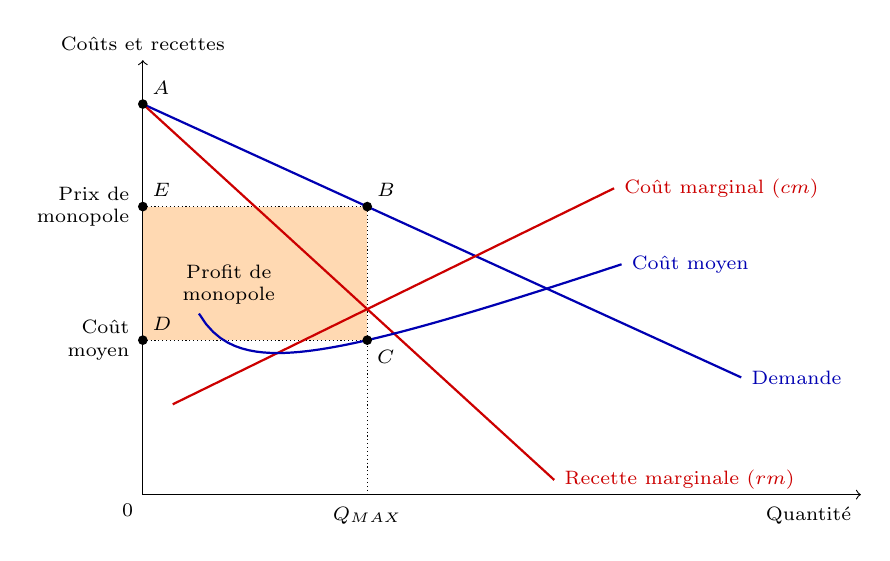
\begin{tikzpicture}[x=0.95cm,y=0.62cm,font=\scriptsize,
      dot/.style={circle,fill=black,inner sep=0pt,minimum size=3.5pt}]
    % profit rectangle
    \fill[orange!30] (0,3.164) rectangle (3,5.9);
    \node[align=center] at (1.15,4.3) {Profit de\\monopole};
    % axes
    \draw[->] (0,0) -- (9.6,0);
    \draw[->] (0,0) -- (0,8.9);
    \node[above] at (0,8.9) {Coûts et recettes};
    \node[below left] at (9.6,-0.05) {Quantité};
    \node[below left] at (0,0) {$0$};
    % guides
    \draw[densely dotted] (0,5.9) -- (3,5.9) -- (3,0);
    \draw[densely dotted] (0,3.164) -- (3,3.164);
    \node[below] at (3,-0.05) {$Q_{\text{MAX}}$};
    \node[left,align=right] at (-0.05,5.9) {Prix de\\monopole};
    \node[left,align=right] at (-0.05,3.164) {Coût\\moyen};
    % curves
    \draw[blue!70!black,thick] (0,8) -- (8,2.4) node[right] {Demande};
    \draw[red!80!black,thick] (0,8) -- (5.5,0.3)
      node[right] {Recette marginale ($rm$)};
    \draw[red!80!black,thick] (0.4,1.85) -- (6.3,6.275)
      node[right] {Coût marginal ($cm$)};
    \draw[blue!70!black,thick] plot[domain=0.75:6.4,samples=60]
      (\x,{0.92+0.55*\x+1.782/\x}) node[right] {Coût moyen};
    % points
    \foreach \p/\l/\a in {(0,8)/A/above right, (3,5.9)/B/above right,
        (3,3.164)/C/below right, (0,3.164)/D/above right, (0,5.9)/E/above right}
      { \node[dot] at \p {}; \node[\a] at \p {$\l$}; }
  \end{tikzpicture}
  \caption*{\small Le profit du monopole. The quantity $Q_{\text{MAX}}$ is set where
  $rm = cm$, the price is read off the courbe de demande, and the shaded rectangle
  $BCDE$ is the profit: profit per unit ($BC$) times units sold ($DC$).}
\end{figure}

\subsubsection{Perte sèche}

The same curves show what the monopole costs society. Because a monopole charges
a price above its coût marginal, some consumers who value the good at more than
it costs to produce do not buy it. The \textbf{quantité de monopole}
(\textit{monopoly quantity}), which the monopole produces and sells, where the
recette marginale meets the coût marginal, is therefore below the \textbf{quantité
efficace} (\textit{efficient quantity}), where the courbe de demande meets the coût
marginal curve.\\

The loss is the \textbf{perte sèche} (\textit{deadweight loss}). It is the area of
the triangle between the courbe de demande, which reflects what the good is worth to
consumers, and the coût marginal curve, which reflects what it costs the
monopole to produce, between the quantité de monopole and the quantité
efficace.

\begin{figure}[h!]
  \centering
  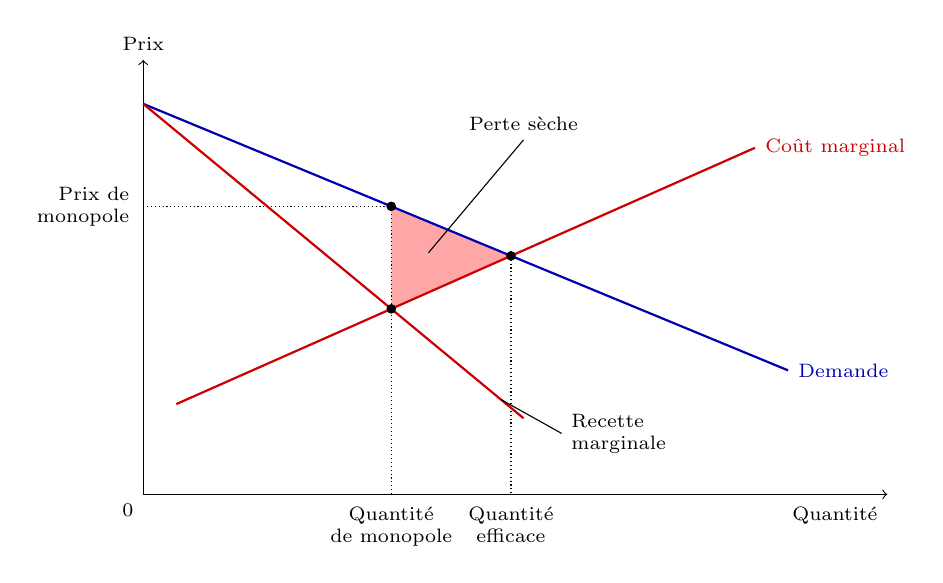
\begin{tikzpicture}[x=1.05cm,y=0.62cm,font=\scriptsize,
      dot/.style={circle,fill=black,inner sep=0pt,minimum size=3.5pt}]
    % deadweight-loss triangle
    \fill[red!35] (3,5.9) -- (3,3.8) -- (4.448,4.886) -- cycle;
    % axes
    \draw[->] (0,0) -- (9,0);
    \draw[->] (0,0) -- (0,8.9);
    \node[above] at (0,8.9) {Prix};
    \node[below left] at (9,-0.05) {Quantité};
    \node[below left] at (0,0) {$0$};
    % guides
    \draw[densely dotted] (0,5.9) -- (3,5.9) -- (3,0);
    \draw[densely dotted] (4.448,4.886) -- (4.448,0);
    \node[left,align=right] at (-0.05,5.9) {Prix de\\monopole};
    \node[below,align=center] at (3,-0.05) {Quantité\\de monopole};
    \node[below,align=center] at (4.448,-0.05) {Quantité\\efficace};
    % curves
    \draw[blue!70!black,thick] (0,8) -- (7.8,2.54) node[right] {Demande};
    \draw[red!80!black,thick] (0,8) -- (4.6,1.56);
    \draw[red!80!black,thick] (0.4,1.85) -- (7.4,7.1)
      node[right] {Coût marginal};
    % labels with leaders
    \node[align=left] (rm) at (5.75,1.25) {Recette\\marginale};
    \draw (rm.west) -- (4.33,1.94);
    \node[align=center] (dwl) at (4.6,7.6) {Perte sèche};
    \draw (dwl.south) -- (3.45,4.95);
    % points
    \foreach \p in {(3,5.9),(3,3.8),(4.448,4.886)}
      \node[dot] at \p {};
  \end{tikzpicture}
  \caption*{\small La perte sèche du monopole. The prix de monopole lies above the
  coût marginal, so the quantité de monopole falls short of the quantité efficace;
  the shaded triangle between the courbe de demande and the coût marginal curve is
  the perte sèche.}
\end{figure}

\subsection{Externalités}

\begin{definition}[Externalités (\textit{externalities})]
  Les \textbf{externalités} sont des effets sur d'autres acteurs économiques non
  pris en compte par le marché.
\end{definition}

They come with either sign, and the course gives examples of each:
\begin{itemize}
  \item \textbf{externalités positives} (\textit{positive externalities}),
    exemples~: éducation $\Longrightarrow$ subsides~; aux États-Unis, le président
    Biden a appelé les États à offrir 100~\$ à chaque Américain nouvellement
    vacciné, en utilisant les fonds de relance fédéraux~;
  \item \textbf{externalités négatives} (\textit{negative externalities})~:
    pollution~;
  \item les deux~: algorithmes et IA (intelligence artificielle) --- gains de
    productivité, crée des emplois~; «~Human downgrading~», détruit des emplois.
\end{itemize}
Two figures develop the first examples of each sign: pollution, in the market for
aluminium, and education.

\begin{figure}[h!]
  \centering
  \begin{tikzpicture}[x=0.55cm,y=0.48cm,font=\scriptsize,>=stealth,
      dot/.style={circle,fill=black,inner sep=0pt,minimum size=3.5pt}]
    \node[font=\footnotesize\bfseries] at (4.7,10.7) {(a) Marché de l'aluminium};
    % axes
    \draw[->] (0,0) -- (9.4,0);
    \draw[->] (0,0) -- (0,9.6);
    \node[left,align=right] at (-0.05,9.3) {Prix de\\l'aluminium};
    \node[below left,align=right] at (9.4,-0.05) {Quantité\\d'aluminium};
    \node[below left] at (0,0) {$0$};
    % curves
    \draw[red!80!black,thick] (0.5,3.35) -- (8.5,8.95)
      node[right,align=left] {Coût social\\(coût privé et\\coût externe)};
    \draw[blue!70!black,thick] (0.5,1.35) -- (8.5,6.95)
      node[right,align=left] {Offre\\(coût privé)};
    \draw[blue!70!black,thick] (0.5,7.625) -- (8.5,1.625)
      node[right,align=left] {Demande\\(valeur privée)};
    % external cost
    \draw[->] (6.8,5.76) -- (6.8,7.66);
    \node[draw,fill=orange!20,align=center] (ec) at (4.9,8.9) {Coût\\externe};
    \draw (ec.east) -- (6.75,7.2);
    % guides and points
    \draw[densely dotted] (3.448,5.414) -- (3.448,0);
    \draw[densely dotted] (4.828,4.379) -- (4.828,0);
    \node[below left,inner xsep=1pt] at (3.448,-0.05) {$Q_{\text{optimum}}$};
    \node[below right,inner xsep=1pt] at (4.828,-0.05) {$Q_{\text{marché}}$};
    \node[dot] at (3.448,5.414) {};
    \node[dot] at (4.828,4.379) {};
    \node (op) at (2.3,7.7) {Optimum};
    \draw (op.south) ++(0.3,0) -- (3.38,5.55);
    \node (eq) at (6.1,2.3) {Équilibre};
    \draw (eq.north) ++(-0.3,0) -- (4.88,4.22);
  \end{tikzpicture}\hspace{0.4cm}%
  \begin{tikzpicture}[x=0.55cm,y=0.48cm,font=\scriptsize,>=stealth,
      dot/.style={circle,fill=black,inner sep=0pt,minimum size=3.5pt}]
    \node[font=\footnotesize\bfseries] at (5.1,10.7) {(b) Éducation};
    % axes
    \draw[->] (0,0) -- (10.2,0);
    \draw[->] (0,0) -- (0,9.6);
    \node[left,align=right] at (-0.05,9.3) {Prix de\\l'éducation};
    \node[below left,align=right] at (10.2,-0.05) {Quantité\\d'éducation};
    \node[below left] at (0,0) {$0$};
    % curves
    \draw[blue!70!black,thick] (0.5,0.9) -- (7.6,6.58)
      node[right,align=left] {Offre\\(coût privé)};
    \draw[blue!70!black,thick] (1,6.8) -- (8,1.9)
      node[below,align=center] {Demande\\(valeur privée)};
    \draw[red!80!black,thick] (9.5,2.85) -- (2.5,7.75)
      node[above,align=center] {Valeur sociale\\(valeur privée et\\bénéfice externe)};
    % external benefit
    \draw[->] (3.5,5.05) -- (3.5,6.95);
    \node[draw,fill=orange!20,align=center] (eb) at (1.75,3.6) {Bénéfice\\externe};
    \draw (eb.north east) -- (3.45,5.9);
    % guides and points
    \draw[densely dotted] (4.667,4.233) -- (4.667,0);
    \draw[densely dotted] (6,5.3) -- (6,0);
    \node[below left,inner xsep=1pt] at (4.667,-0.05) {$Q_{\text{marché}}$};
    \node[below] at (6,-0.05) {$Q_{\text{optimum}}$};
    \node[dot] at (4.667,4.233) {};
    \node[dot] at (6,5.3) {};
    \node (eq) at (3.1,1.1) {Équilibre};
    \draw (eq.north east) -- (4.6,4.1);
    \node (op) at (7.7,5.3) {Optimum};
    \draw (op.west) -- (6.1,5.3);
  \end{tikzpicture}
  \caption*{\small Externalités négatives et positives~: (a) le marché de
  l'aluminium, (b) l'éducation. In (a) the coût social curve lies above the courbe
  d'offre by the coût externe, so $Q_{\text{optimum}}$ is smaller than
  $Q_{\text{marché}}$; in (b) the valeur sociale curve lies above the courbe de
  demande by the bénéfice externe, so $Q_{\text{optimum}}$ is larger than
  $Q_{\text{marché}}$.}
\end{figure}

\subsubsection{Externalités négatives : marché de l'aluminium avec/sans externalités}

The figure sets the market for aluminium with and without its externalité. The
courbe d'offre reflects the producers' \textbf{coût privé} (\textit{private
cost}). Producing aluminium pollutes, which adds a \textbf{coût externe}
(\textit{external cost}), borne by others. The \textbf{coût social}
(\textit{social cost}) is the coût privé plus the coût externe: a curve lying above
the courbe d'offre, the gap between them being the coût externe.\\

The market settles at its équilibre, where demand meets supply, at the quantity
$Q_{\text{marché}}$. The \textbf{optimum social} (\textit{social optimum}) is where
demand meets the coût social curve, at $Q_{\text{optimum}}$. With an externalité
négative such as pollution, the coût social of the good exceeds its coût privé, so
$Q_{\text{optimum}}$ is smaller than $Q_{\text{marché}}$: the market produces more
aluminium than the optimum.

\subsubsection{Externalités positives : éducation}

Education is the reverse case. The courbe d'offre reflects the coût privé of
providing it, and the courbe de demande the \textbf{valeur privée}
(\textit{private value}) of education to those who acquire it. Education also
brings a \textbf{bénéfice externe} (\textit{external benefit}), and the
\textbf{valeur sociale} (\textit{social value}) is the valeur privée plus the
bénéfice externe: a curve lying above the courbe de demande, the gap between them
being the bénéfice externe.\\

The équilibre is where demand meets supply, at $Q_{\text{marché}}$; the optimum is
where the valeur sociale curve meets supply, at $Q_{\text{optimum}}$. With an
externalité positive, the valeur sociale of the good exceeds its valeur privée, so
$Q_{\text{optimum}}$ is larger than $Q_{\text{marché}}$. This is the case the
examples above sum up as «~éducation $\Longrightarrow$ subsides~».

\subsubsection{Solution 1 : réglementation}

Three solutions to pollution follow. The first is réglementation~: «~Certains
usages sont simplement interdits~».
\begin{itemize}
  \item Exemple~: zones à faibles émissions (ZFE), vignettes Crit'Air.
  \item Exemple~: interdiction de PL (poids lourds) certains jours.
\end{itemize}

\subsubsection{Solution 2 : l'approche de Pigou}

The second solution is to «~faire payer en fonction de la pollution~», the
principle of the \textbf{pollueur-payeur} (\textit{polluter-pays principle}),
«~et imposer une \textbf{taxe pigouvienne}~» (\textit{Pigouvian tax}). It meets
problems, and the first is stated outright: «~Problème \#1~: ce sont les plus
pauvres qui paient~».

\paragraph{Effets redistributifs.} The first problem is that of the
\textbf{effets redistributifs} (\textit{redistributive effects}) of the tax. Two
pictures make the point. In a cartoon, an economist lists the benefits of a
plan to an environmental protester --- less dependence on oil imports, less
wasteful consumption, lower greenhouse emissions, alternative fuels --- and the
protester welcomes each one and presses to hear the plan, until it turns out to be
a higher price of petrol at the pump (3,49~\$ a gallon), and the protester rejects it. A
photograph shows a crowd of protesters in yellow high-visibility vests under a
banner «~NON AUX TAXES~».

\paragraph{Autres problèmes.} Three more problems are posed, and left open:
\begin{itemize}
  \item deuxième problème~: faire payer en fonction de la pollution~?
  \item troisième problème~: comment calculer la pollution~?
  \item quatrième problème~: comment estimer la disponibilité à payer des gens
    pour régler les problèmes de pollution~?
\end{itemize}

\subsubsection{Solution 3 : cap and trade systems}

The third solution is a market: «~Transfert volontaire du \textbf{droit à
polluer}~» (\textit{pollution rights}), exemple~: EU ETS. Three claims come with
it:
\begin{itemize}
  \item les entreprises qui font une transaction doivent y trouver leur compte~;
  \item le marché garantit un équilibre efficient~;
  \item les entreprises internalisent l'externalité.
\end{itemize}

\begin{figure}[h!]
  \centering
  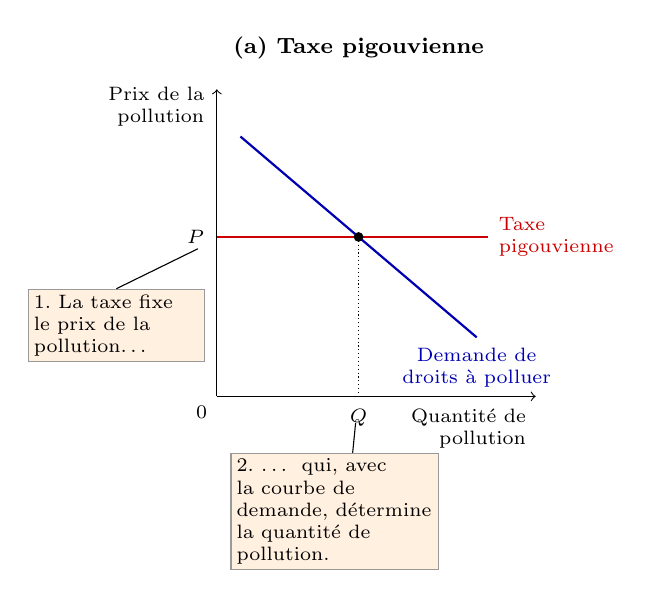
\begin{tikzpicture}[x=0.75cm,y=0.75cm,font=\scriptsize,
      dot/.style={circle,fill=black,inner sep=0pt,minimum size=3.5pt},
      call/.style={draw=black!40,fill=orange!12,align=left,text width=2.1cm,
        inner sep=2pt,execute at begin node={\hyphenpenalty=10000}}]
    \node[font=\footnotesize\bfseries] at (2.4,5.9) {(a) Taxe pigouvienne};
    % axes
    \draw[->] (0,0) -- (5.4,0);
    \draw[->] (0,0) -- (0,5.2);
    \node[left,align=right] at (-0.05,4.9) {Prix de la\\pollution};
    \node[below left,align=right] at (5.4,-0.05) {Quantité de\\pollution};
    \node[below left] at (0,0) {$0$};
    % demand and tax
    \draw[blue!70!black,thick] (0.4,4.4) -- (4.4,1.0)
      node[below,align=center] {Demande de\\droits à polluer};
    \draw[red!80!black,thick] (0,2.7) -- (4.6,2.7)
      node[right,align=left] {Taxe\\pigouvienne};
    \draw[densely dotted] (2.4,2.7) -- (2.4,0);
    \node[dot] at (2.4,2.7) {};
    \node[left] at (-0.05,2.7) {$P$};
    \node[below] at (2.4,-0.05) {$Q$};
    % callouts
    \node[call] (a1) at (-1.7,1.2)
      {1.~La taxe fixe le prix de la pollution\ldots};
    \draw (a1.north) -- (-0.32,2.5);
    \node[call,text width=2.5cm] (a2) at (2.0,-1.95)
      {2.~\ldots{} qui, avec la courbe de demande, détermine la quantité de
      pollution.};
    \draw (a2.north) ++(0.3,0) -- (2.35,-0.45);
  \end{tikzpicture}\hspace{0.6cm}%
  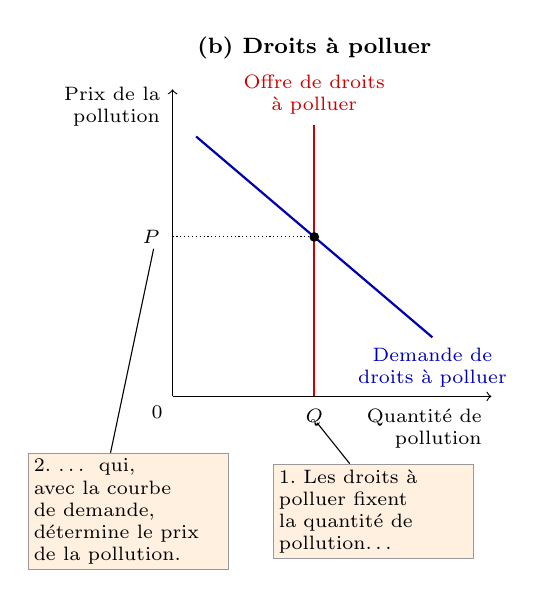
\begin{tikzpicture}[x=0.75cm,y=0.75cm,font=\scriptsize,
      dot/.style={circle,fill=black,inner sep=0pt,minimum size=3.5pt},
      call/.style={draw=black!40,fill=orange!12,align=left,text width=2.4cm,
        inner sep=2pt,execute at begin node={\hyphenpenalty=10000}}]
    \node[font=\footnotesize\bfseries] at (2.4,5.9) {(b) Droits à polluer};
    % axes
    \draw[->] (0,0) -- (5.4,0);
    \draw[->] (0,0) -- (0,5.2);
    \node[left,align=right] at (-0.05,4.9) {Prix de la\\pollution};
    \node[below left,align=right] at (5.4,-0.05) {Quantité de\\pollution};
    \node[below left] at (0,0) {$0$};
    % demand and permits
    \draw[blue!70!black,thick] (0.4,4.4) -- (4.4,1.0)
      node[below,align=center] {Demande de\\droits à polluer};
    \draw[red!80!black,thick] (2.4,0) -- (2.4,4.6)
      node[above,align=center] {Offre de droits\\à polluer};
    \draw[densely dotted] (0,2.7) -- (2.4,2.7);
    \node[dot] at (2.4,2.7) {};
    \node[left] at (-0.05,2.7) {$P$};
    \node[below] at (2.4,-0.05) {$Q$};
    % callouts
    \node[call] (b2) at (-0.75,-1.95)
      {2.~\ldots{} qui, avec la courbe de demande, détermine le prix de la
      pollution.};
    \draw (b2.north) ++(-0.3,0) -- (-0.32,2.5);
    \node[call] (b1) at (3.4,-1.95)
      {1.~Les droits à polluer fixent la quantité de pollution\ldots};
    \draw (b1.north) ++(-0.4,0) -- (2.45,-0.45);
  \end{tikzpicture}
  \caption*{\small Comparaison~: taxe pigouvienne et droits à polluer. The tax fixes
  the price and lets demand set the quantity; the droits à polluer fix the quantity
  and let demand set the price. The price $P$ and the quantity $Q$ of pollution are
  the same in both panels.}
\end{figure}

\paragraph{Comparaison.} The figure sets the taxe pigouvienne of Solution 2 against
the droits à polluer of Solution 3, with the same demand for droits à polluer in
both panels. In panel (a), the public authority sets a price on pollution by
levying the tax, and the courbe de demande determines the quantity of pollution. In
panel (b), it limits the quantity of pollution by limiting the number of droits à
polluer, and the courbe de demande determines the price of pollution. The price and the
quantity of pollution are the same in the two cases.

\paragraph{Critiques.} The course lists four critiques of the cap and trade
systems:
\begin{itemize}
  \item légitime la pollution~: utilisé pour des raisons de profits, pas pour
    diminuer la pollution~;
  \item nécessite une gouvernance très forte pour éviter la fraude, la
    manipulation des prix et la collusion~;
  \item \emph{Forum shopping}~: délocalise dans les zones géographiques où il y a
    moins de contraintes environnementales~; donne un avantage concurrentiel~;
  \item favorise le statu quo vs.\ innovation environnementale.
\end{itemize}

\subsection{Biens publics et biens communs}

\subsubsection{Les biens publics}

The \textbf{biens publics} (\textit{public goods}) are placed in a typologie des
biens économiques, which sorts goods by two characteristics. A good has
\textbf{excluabilité} (\textit{excludability}) when people can be kept from using
it, and \textbf{rivalité} (\textit{rivalry}) in consumption when one person's use
of it reduces what others can use.\\

The two yes-or-no questions give four categories: the \textbf{biens privés}
(\textit{private goods}), excludable and rival; the \textbf{biens de club}
(\textit{club goods}), excludable but not rival; the biens communs, rival but not
excludable, which return at the end of this subsection; and the biens publics,
neither excludable nor rival.

\begin{table}[h!]
  \centering
  \small
  \begin{tabularx}{\textwidth}{@{}l>{\raggedright\arraybackslash}X%
      >{\raggedright\arraybackslash}X@{}}
    \toprule
    & \multicolumn{2}{c}{Rivalité dans la consommation~?} \\
    \cmidrule(l){2-3}
    Excluabilité~? & Oui & Non \\
    \midrule
    Oui & \textit{Biens privés}~: cornets de glace~; vêtements~; routes à péage
          encombrées
        & \textit{Biens de club}~: protection contre les incendies~; télévision
          par câble~; routes à péage non encombrées \\
    \addlinespace
    Non & \textit{Biens communs}~: poissons dans l'océan~; l'environnement~;
          routes gratuites encombrées
        & \textit{Biens publics}~: sirène d'alerte aux tornades~; défense
          nationale~; routes gratuites non encombrées \\
    \bottomrule
  \end{tabularx}
  \caption*{\small Typologie des biens économiques. Goods sorted by excluabilité
    (rows) and rivalité in consumption (columns), with three examples in each
    category.}
\end{table}

\paragraph{Remarques.} «~Les frontières ne sont pas toujours très claires~»; two
examples:
\begin{itemize}
  \item \textbf{effets de congestion} (\textit{congestion effects}) ---
    \textbf{biens publics impurs} (\textit{impure public goods})~: hôpitaux
    durant le covid~;
  \item \textbf{coût de l'excluabilité} (\textit{cost of exclusion})~:
    exemple, autoroutes payantes dans certains pays de l'UE.
\end{itemize}

\subsubsection{Biens publics : efficacité économique}

Three points bear on the efficiency of the biens publics:
\begin{itemize}
  \item problème du \textbf{passager clandestin} (\textit{free rider}) qui
    profite du service public sans payer, problème qui provient de la
    non-excluabilité~;
  \item de plus, très souvent, le bien public est associé à des externalités
    positives --- exemple~: recherche fondamentale~;
  \item conséquences~: \textbf{sous-investissement} (\textit{underinvestment}) du
    secteur privé = défaillance de marché --- les entreprises ne peuvent pas
    s'accaparer l'ensemble du surplus social qu'elles créent.
\end{itemize}

\subsubsection{Les biens communs}

The \textbf{biens communs} (\textit{common resources}) are the rival goods from
which no one can be excluded. Their problem has a name:

\begin{definition}[Tragédie des communs (\textit{tragedy of the commons})]
  La ressource commune est détruite par l'action individuelle.
\end{definition}

\begin{example}[Ressources communes détruites]
  Banc de poissons, pâturage.
\end{example}

«~Il existe des solutions~». Two are named, and not developed:
\begin{itemize}
  \item Elinor Ostrom~;
  \item droits de propriété --- and with them the tragédie des anti-communs, for
    which the documentary «~The Internet's Own Boy: The Story of Aaron Swartz~»
    is given.
\end{itemize}

\subsection{Asymétries d'information}

\subsubsection{Problèmes informationnels : lemons}

The last défaillance de marché comes from what buyers cannot know. The example is
Akerlof's, on used cars.

\begin{example}[Les lemons d'Akerlof~: voitures d'occasion]
  The market is set up as follows.
  \begin{itemize}
    \item 100 vendeurs, 100 acheteurs~;
    \item 50~\% des voitures sont des «~\textbf{prunes}~» (\textit{plums}),
      50~\% des «~\textbf{citrons}~» (\textit{lemons})~; les acheteurs ne
      peuvent pas vérifier la qualité de la voiture (asymétries
      d'information)~;
    \item les vendeurs de lemons demandent 1\,000~\$, ceux de plums
      2\,000~\$~;
    \item les acheteurs sont prêts à payer 1\,200~\$ et 2\,400~\$
      respectivement~;
    \item disponibilité moyenne à payer = 1\,800~\$.
  \end{itemize}
  Since buyers cannot tell the two kinds apart, what they will pay for a car is
  this average: half the cars are lemons and half plums, and 1\,800~\$ is the
  average of 1\,200~\$ and 2\,400~\$.\\

  Problème~: les vendeurs de plums ne sont pas prêts à vendre à ce prix, which
  is below the 2\,000~\$ they ask.
  \begin{itemize}
    \item Les acheteurs savent qu'il ne reste que des lemons sur le marché et ils
      ne sont prêts à payer que 1\,200~\$, pas 1\,800~\$~;
    \item le marché s'effondre~: il n'y a plus que des lemons sur le marché~;
    \item l'asymétrie d'information crée une externalité entre les «~mauvais~»
      et les «~bons~» vendeurs.
  \end{itemize}
\end{example}

De manière plus générale~: un problème de confiance dans le marché.
